\documentclass[a4paper,10pt]{article}

\usepackage{ucs}
\usepackage[utf8]{inputenc}
\usepackage{amsmath}
\usepackage{babel}
\usepackage{fontenc}
\usepackage{graphicx}

\usepackage[dvips]{hyperref}

\date{22/05/2019}

\begin{document}
 \section{Stato dell'arte}
 \subsection{Andy M. Sarroff, Dartmouth college}
 \subsection{Nils M$\ddot{o}$nning \& Suresh Manandhar, University of York}
 Nils M$\ddot{o}$nning e Suresh Manandhar hanno comparato diversi MLP (multi layer perceptron) complessi con dei corrispettivi MLP reali. Per evitare casistiche particolari sono stati utilizzati 4 database differenti (MNIST digit classification, CIFAR-10 image classification, CIFAR-100 image classification, Reuters topic classification) e per ridurre l'impatto delle inizializzazioni, ogni modello ha effettuato 10 training. \'E tenuto fisso il numero di elementi per layer (64 neuroni nel caso reale e 32 in quello complesso) e per il calcolo del gradiente nel caso complesso è stato utilizzato Wirtinger. I risultati ottenuti sono mostrati nelle tabelle seguenti:
 
 
 Tabella 1) Test di MLP con $k$ + 2 layers, ognuno di 64 elementi (64 neuroni per la rete reale e 32 per quella complessa) e output di 10 elementi.
 
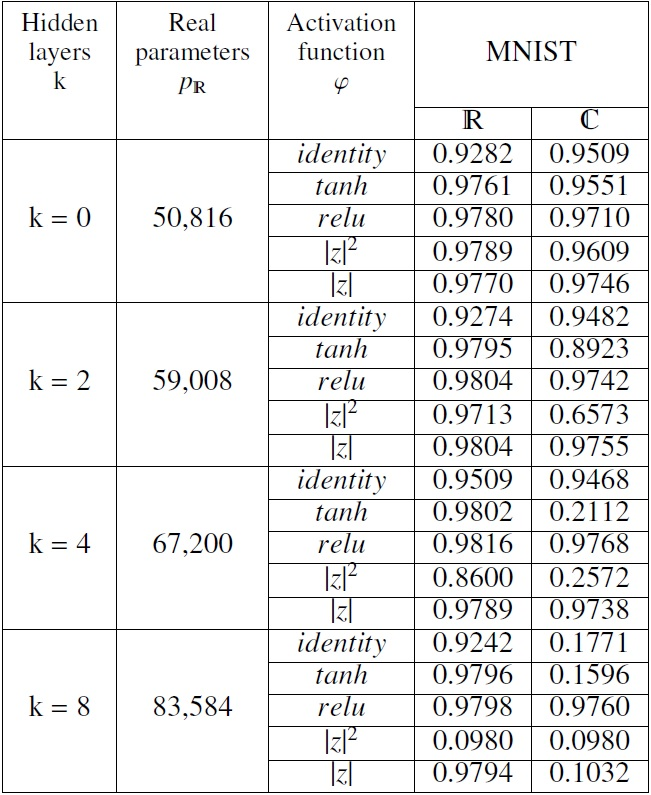
\includegraphics[width=%
\textwidth]{tabella1}


Tabella 2) Test di MLP con $k$ + 2 layers, ognuno di 64 elementi (64 neuroni per la rete reale e 32 per quella complessa) e output di 46 elementi.

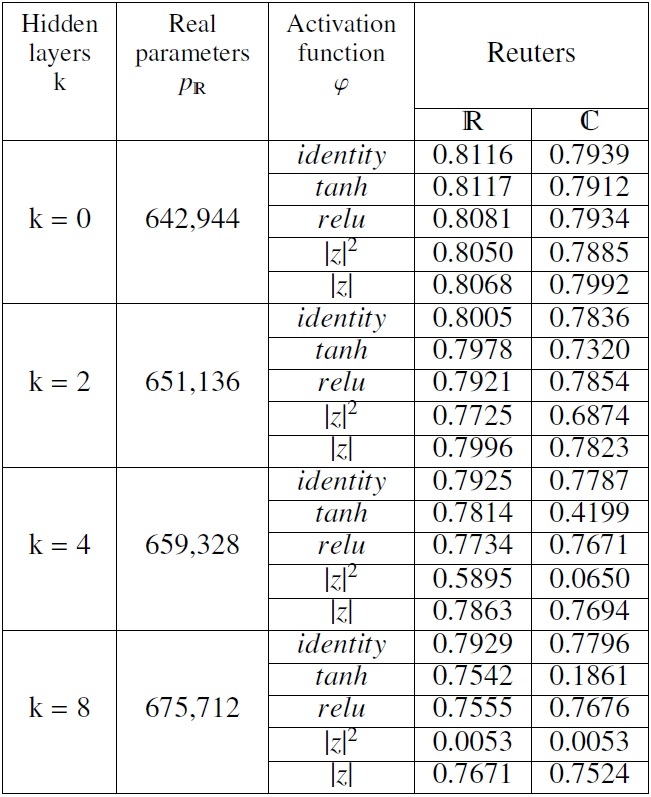
\includegraphics[width=%
\textwidth]{tabella2}


Tabella 3) Test di MLP con $k$ + 2 layers, ognuno di 128 elementi (128 neuroni per la rete reale e 64 per quella complessa) e output di 10 elementi.

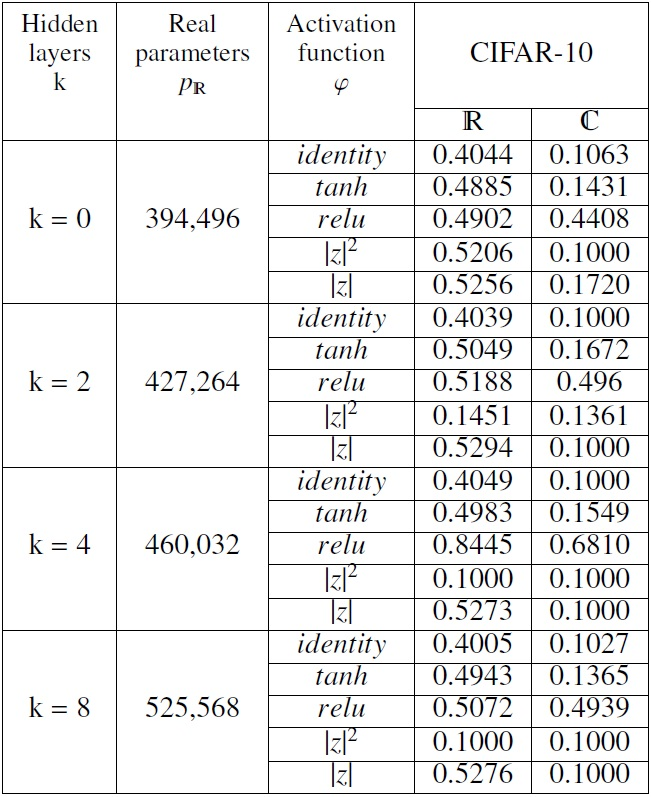
\includegraphics[width=%
\textwidth]{tabella3}


Tabella 4) Test di MLP con $k$ + 2 layers, ognuno di 128 elementi (128 neuroni per la rete reale e 64 per quella complessa) e output di 100 elementi.

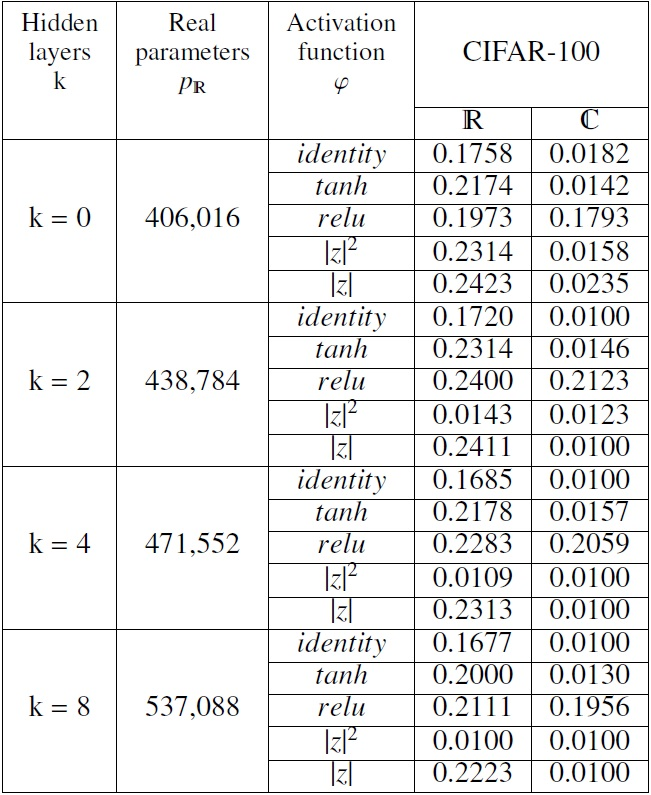
\includegraphics[width=%
\textwidth]{tabella4}


Tabella 5) Test di MLP con $k$ + 2 layers, 500000 parametri reali e output di 10 elementi.

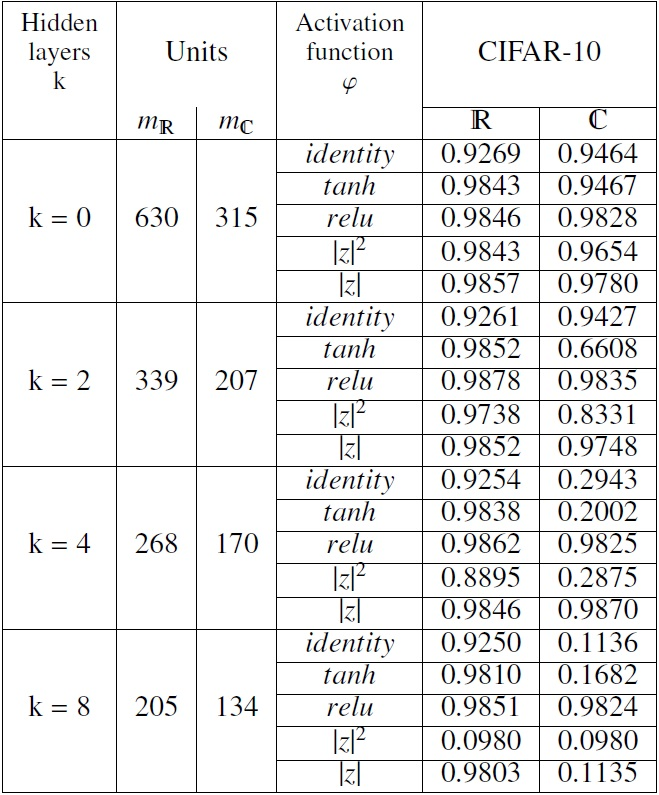
\includegraphics[width=%
\textwidth]{tabella5}


Tabella 6) Test di MLP con $k$ + 2 layers, 500000 parametri reali e output di 46 elementi.

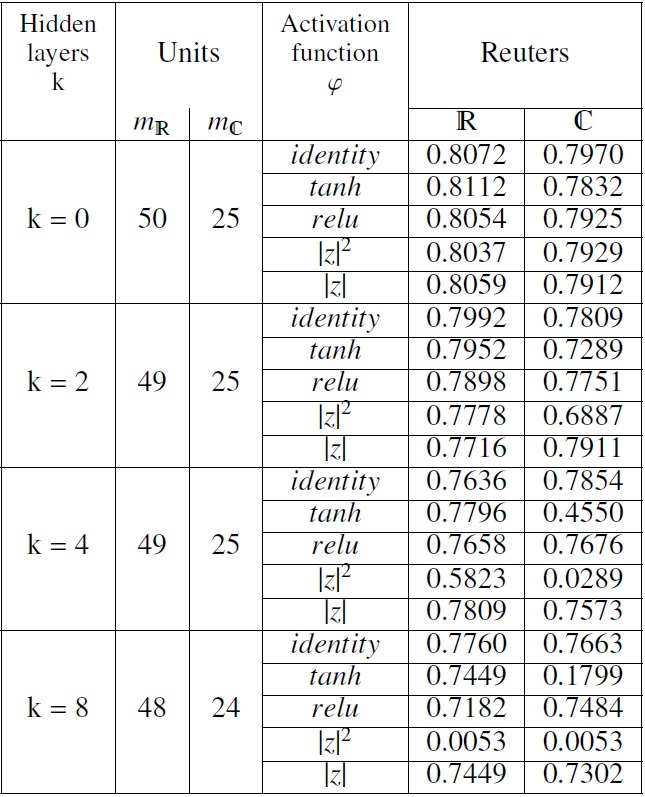
\includegraphics[width=%
\textwidth]{tabella6}


Tabella 7) Test di MLP con $k$ + 2 layers, 500000 parametri reali e output di 10 elementi.

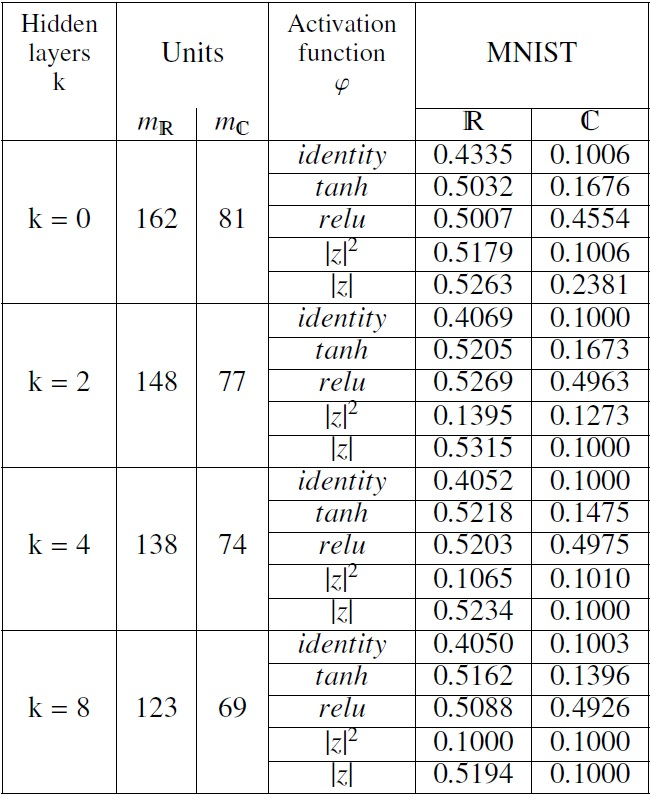
\includegraphics[width=%
\textwidth]{tabella8}


Tabella 8) Test di MLP con $k$ + 2 layers, 500000 parametri reali e output di 100 elementi.

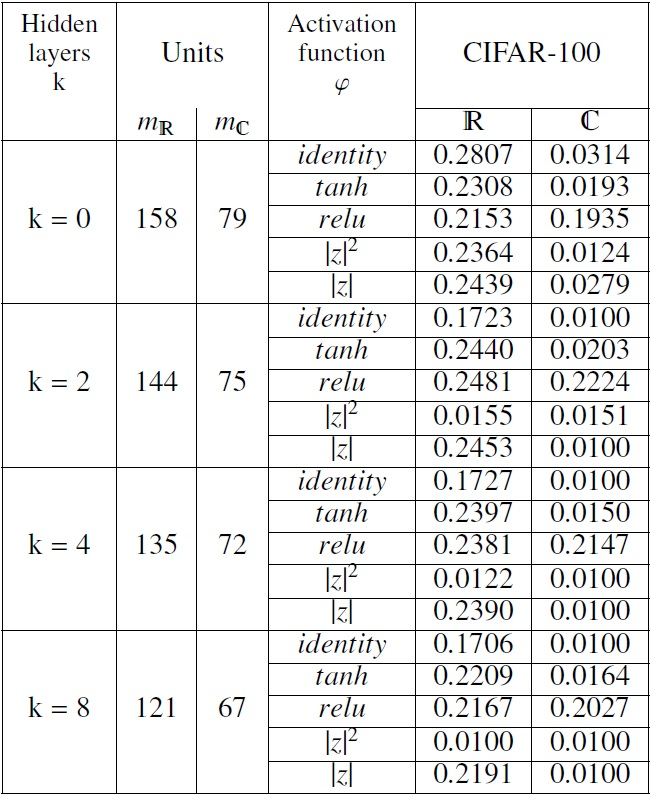
\includegraphics[width=%
\textwidth]{tabella9}
 
 \subsection{Nitzan Guberman}
 
 Viene costruita una CNN (convolutional neural network) complessa per determinare se una determinata patch di immagine contiene una cellula e confrontare questa rete con la sua controparte reale. Le due reti mostrano risultati comparabili, sebbene la rete complessa soffra di difficoltà di convergenza. Per verificare l'affermazione che le CNN complesse agiscano come regolarizzatori, esaminiamo il comportamento della $loss$ $funtion$. La CNN con valore reale è significativamente più vulnerabile all'overfitting. Confrontiamo la rete complessa con il suo equivalente reale. Questa rete condivide la stessa architettura di quella complessa, solo con il doppio dei canali e dei kernel di convoluzione. Per costruzione, l'ultimo strato della rete reale è costituito da un numero doppio di neuroni rispetto a quello complesso. Poiché le etichette sono binarie, il livello finale deve essere a due canali, quindi aggiungiamo un affine layer completamente connesso che sostituisce il livello di proiezione nella rete complessa. 
 
 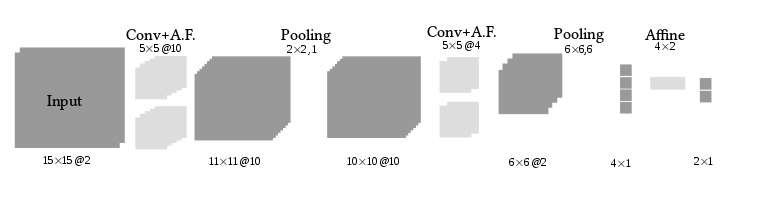
\includegraphics[width=%
\textwidth]{RCNN}

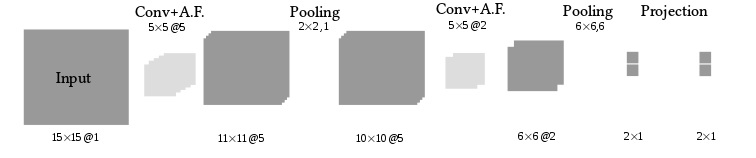
\includegraphics[width=%
\textwidth]{CCNN}

+ eventualmente risultati reti neurali complesse senza confronto con caso reale



\end{document}
